\documentclass{article}
\usepackage[inline-math]{chs-physics-report}
\usepackage{float}
\usepackage{pgfplots}
\usepackage{pgfplotstable}
\usepackage{booktabs}

\pgfplotsset{compat=1.18}

\title{2.1: Friction Lab}
\name{Gavin Chen}
\ww{Cole TerBush and Daniel Aronov}

\begin{document}
\maketitle

\section{Free Body Diagrams and Derivations}
\subsection{Section 1}
\subsubsection{Free body Diagram}
\begin{center}
    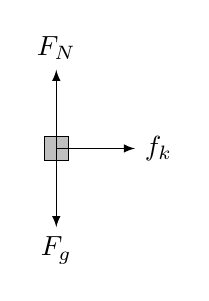
\begin{tikzpicture}[force/.style={>=latex},m/.style={rectangle,draw=black,fill=lightgray,minimum size=0.3cm,thin}]
        \node[m] (m) {};
        \draw [force,->] (m.center) -- ++(0,-1) node[below] {$F_g$};
        \draw [force,->] (m.center) -- ++(0,1) node[above] {$F_N$};
        \draw [force,->] (m.center) -- ++(1,0) node[right] {$f_k$};
    \end{tikzpicture}
\end{center}
\subsubsection{Derivation}
\[{v_x}^2 = {{v_x}_0}^2 + 2a_x\Delta x\]
\[a_x = \frac{{v_x}^2 - {{v_x}_0}^2}{2\Delta x} = \frac{f_k}{m} = \frac{\mu_k mg}{m}\]
\[\mu_k g = \frac{{v_x}^2 - {{v_x}_0}^2}{2\Delta x}\]
\[\mu_k = \frac{{v_x}^2 - {{v_x}_0}^2}{2g\Delta x}\]
Since the final velocity is zero, this can be simplified to:
\[\mu_k = \frac{-{{v_x}_0}^2}{2g\Delta x}\]

\subsection{Section 2}
\subsubsection{Free Body Diagram}
\begin{center}
    \begin{tikzpicture}[force/.style={>=latex},m/.style={rectangle,draw=black,fill=lightgray,minimum size=0.3cm,thin}]
        \node[m] (m) {};
        \draw [force,->] (m.south) -- ++(0,-1) node[below] {$F_g$};
        \draw [force,->] (m.south) -- ++(0,1) node[above] {$F_N$};
        \draw [force,->] (m.west) -- ++(-2,0) node[left] {$f_s$};
        \draw [force,->] (m.west) -- ++(2,0) node[right] {$F_{app}$};
    \end{tikzpicture}
\end{center}

\begin{center}
    \begin{tikzpicture}[force/.style={>=latex},m/.style={rectangle,draw=black,fill=lightgray,minimum size=0.3cm,thin}]
        \node[m] (m) {};
        \draw [force,->] (m.south) -- ++(0,-1) node[below] {$F_g$};
        \draw [force,->] (m.south) -- ++(0,1) node[above] {$F_N$};
        \draw [force,->] (m.west) -- ++(-2,0) node[left] {$f_k$};
        \draw [force,->] (m.west) -- ++(2,0) node[right] {$F_{app}$};
    \end{tikzpicture}
\end{center}

\subsubsection{Derivation}
At peak static friction:
\[f_s = \mu_sF_n = \mu_smg\]
\[\mu_s = \frac{f_s}{mg}\]
At kinetic friction:
\[f_k = \mu_kF_n = \mu_kmg\]
\[\mu_k = \frac{f_k}{mg}\]

\subsection{Section 3}
\subsubsection{Free Body Diagram}
\begin{center}
    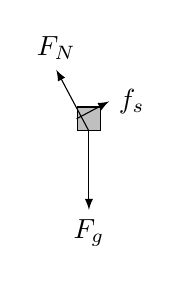
\begin{tikzpicture}[force/.style={>=latex},m/.style={rectangle,draw=black,fill=lightgray,minimum size=0.3cm,thin}]
        \node[m] (m) {};
        \draw [force,->] (m.south) -- ++(0,-1) node[below] {$F_g$};

        \begin{scope}[rotate=28]
            \draw [force,->] (m.south) -- ++(0,{cos(28)}) node[above] {$F_N$};
            \draw [force,->] (m.west) -- ++({sin(28)},0) node[right] {$f_s$};

        \end{scope}
    \end{tikzpicture}
\end{center}

\subsubsection{Derivation}
At the point right before the box starts to fall:
\[f_s = \mu_sF_n = \mu_smg\cos(\theta) = mg\sin(\theta)\]
\[\mu_s = \tan(\theta)\]

\section{Data}
\subsection{Section 1}
\begin{center}
    \pgfplotstabletypeset[col sep=comma, /pgf/number format/fixed, fixed zerofill, precision=2, every head row/.style={
                before row={
                        \toprule
                    },
                after row={
                        \bottomrule
                    },
            },
        every last row/.style={
                after row=\bottomrule
            }]{Section 1.csv}
\end{center}

\subsection{Section 2}
\begin{center}
    \pgfplotstabletypeset[col sep=comma, /pgf/number format/fixed, fixed zerofill, precision=3, string type, column type=c, columns/{lowlevel colname}/.style={column name = display column name},every head row/.style={
                before row={
                        \toprule
                    },
                after row={
                        \bottomrule
                    },
            },
        every last row/.style={
                after row=\bottomrule
            }]{Section 2.csv}
\end{center}

\subsection{Section 3}
\begin{center}
    \pgfplotstabletypeset[col sep=comma, /pgf/number format/fixed, fixed zerofill, precision=3, every head row/.style={
                before row={
                        \toprule
                    },
                after row={
                        \bottomrule
                    },
            },
        every last row/.style={
                after row=\bottomrule
            }]{Section 3.csv}
\end{center}
\section{$\mu$ Values}
\subsection{Section 1}
\[{\mu_k}_1 = 0.42\]
\subsection{Section 2}
\[{\mu_k}_2 = 0.265\]
\[{\mu_s}_2 = 0.421\]
\subsection{Section 3}
\[{\mu_s}_3 = 0.537\]

\subsection{Comparison}
Our values for both coefficients were very inconsistent, with $\mu_k$ having a difference of 0.155 and $\mu_s$ having a difference of 0.116. This should not happen, as we conducted the lab on the same surface for all three sections. As such, these inconsistencies may have been a result of experimental error.

\section{Improvements}
For Section 2, we had different people pull for each trial, which definitely skewed our results. Having one person pull would be better, as it results in more consistency. For Section 3, we only had enough time to perform one trial, but if we had more time, we definitely should have performed more trials. If we had more time, we would also redo some of the sections entirely, since the value for each coefficient of friction vary drastically between each section when they should not vary much.
\end{document}